\documentclass{article}
\usepackage{authblk}
\usepackage[utf8]{vietnam}
\usepackage[margin=1in]{geometry}
\usepackage[utf8]{inputenc}
\usepackage{multicol}
\usepackage{natbib}
\usepackage{graphicx}

\title{%
  Các mô hình ước tính phù hợp khi dữ liệu còn hạn chế \\
  \large Dự đoán tổng số ca mắc SARS-COV-2 tại Việt Nam theo dòng thời gian}

%\title{Các mô hình ước tính phù hợp khi dữ liệu còn hạn chế}
\date{}

\author[1]{\small Anh H. Ngo}
\author[2]{\small Nam T. Hoang}
\author[3]{\small Khoi T. Nguyen}

\affil[1]{\footnotesize École Polytechnique, Institut Polytechnique de Paris, FRANCE}
\affil[2]{\footnotesize Department of Mathematics and Computer Science, Beloit College, USA 53511}
\affil[3]{\footnotesize Melbourne School of Engineering, The University of Melbourne, Parkville, Victoria, AUSTRALIA 3052}



\begin{document}

\maketitle

\section{Lời mở đầu}

\subsection{Hiện trạng}
Ở thời điểm hiện tại trong quá trình chống dịch tại Việt Nam, có rất nhiều dữ liệu đã thu thập được. Tuy nhiên, những dữ liệu này lại chưa được trích xuất một cách hoàn chỉnh, phần lớn là untidied data, có nghĩa là các dữ liệu lộn xộn, không thống nhất về hình thức cũng như nội dung. Từ vấn đề này, các nghiên cứu sinh ra nhu cầu sử dụng ít dữ liệu, nhưng có khả năng dự đoán nhanh các số liệu. 

\subsection{Yêu cầu}
Để đáp ứng được nhu cầu nêu trên, cần phải thỏa mãn 3 yêu cầu chính:

\begin{itemize}
    \item Tốc độ nhanh chóng
    \item Có độ chính xác cao
    \item Mang ý nghĩa thực tiễn
\end{itemize}

\section{Giải pháp}
Để đáp ứng được các yêu cầu đã nêu, hiện tại có các giải pháp như sau:

\begin{itemize}
    \item Xây dựng mô hình mang số lượng biến số tối thiểu.
    \item Độ phức tạp mô hình đủ cao, nhưng không bị overfit (quá bám sát các dữ liệu đã có và tạo ra độ thiếu chính xác trong việc dự đoán).
\end{itemize}

$\Rightarrow$ Có thể áp dụng mô hình 1-dimensinoal (1 biến số), dựa trên số ca đã có từ dữ liệu của các ngày trước đó.

\begin{multicols}{2}

\subsection{Ưu điểm}
\begin{itemize}
    \item Nhanh chóng
    \item Độ chính xác cao
\end{itemize}

$\Rightarrow$ \textbf{Đủ ý nghĩa để đưa ra giải pháp vĩ mô kịp thời.}
\columnbreak

\subsection{Nhược điểm}
\begin{itemize}
    \item Không mang ý nghĩa dịch tễ, do chỉ xác định được là nhiễm, chưa xác định được nguồn lây, F1,...
    \item Độ chính xác chưa đạt tuyệt đối. Sai số dao động ở mức 3-5\%.
\end{itemize}

$\Rightarrow$ \textbf{Sẽ cải thiện được bằng nhiều dữ liệu biến khác nhau.}
\end{multicols}

\pagebreak

\section{Tiếp cận ban đầu}

Các giải pháp để tạo nên bước đi đầu tiên sẽ được áp dụng từ các phương pháp trong 2 lĩnh vực:

\subsection{Traditional Machine Learning}

Lĩnh vực máy học truyền thống có thể được áp dụng thông qua những phương pháp sau:

\begin{itemize}
    \item Convolutional Neural Network (CNN)
    \item Long Short-term Memory (LSTM)
    \item ARIMA family
\end{itemize}

\subsection{Mô hình toán học}

Để áp dụng bằng các mô hình, có thể sử dụng mô hình Grey và các bản mở rộng (Grey Model and extensions).

\section{ Mô hình Machine Learning truyền thống}

\subsection{Phân loại}
Các mô hình Machine Learning truyền thống được áp dụng bao gồm:

\begin{itemize}
    \item Neural network
    \begin{itemize}
        \item Dựa trên mạng neural thần kinh của con người.
        \item CNN có nhiều mạng và neural ẩn để học tốt hơn các mạng máy học đơn thuần.
        \item LSTM có nhiều cell (tế bào), hoạt động như bộ não của con người ,có chức năng “quên" để lọc data.
        \item Biến thể Bidirectional LSTM (BiLSTM) có khả năng học từ hai chiều (input và output). 
    \end{itemize}
    \item ARIMA Family
    Là mô hình xác suất cơ bản, được dùng để benchmark các mô hình khác.
\end{itemize}

    \begin{figure}
    \centering
    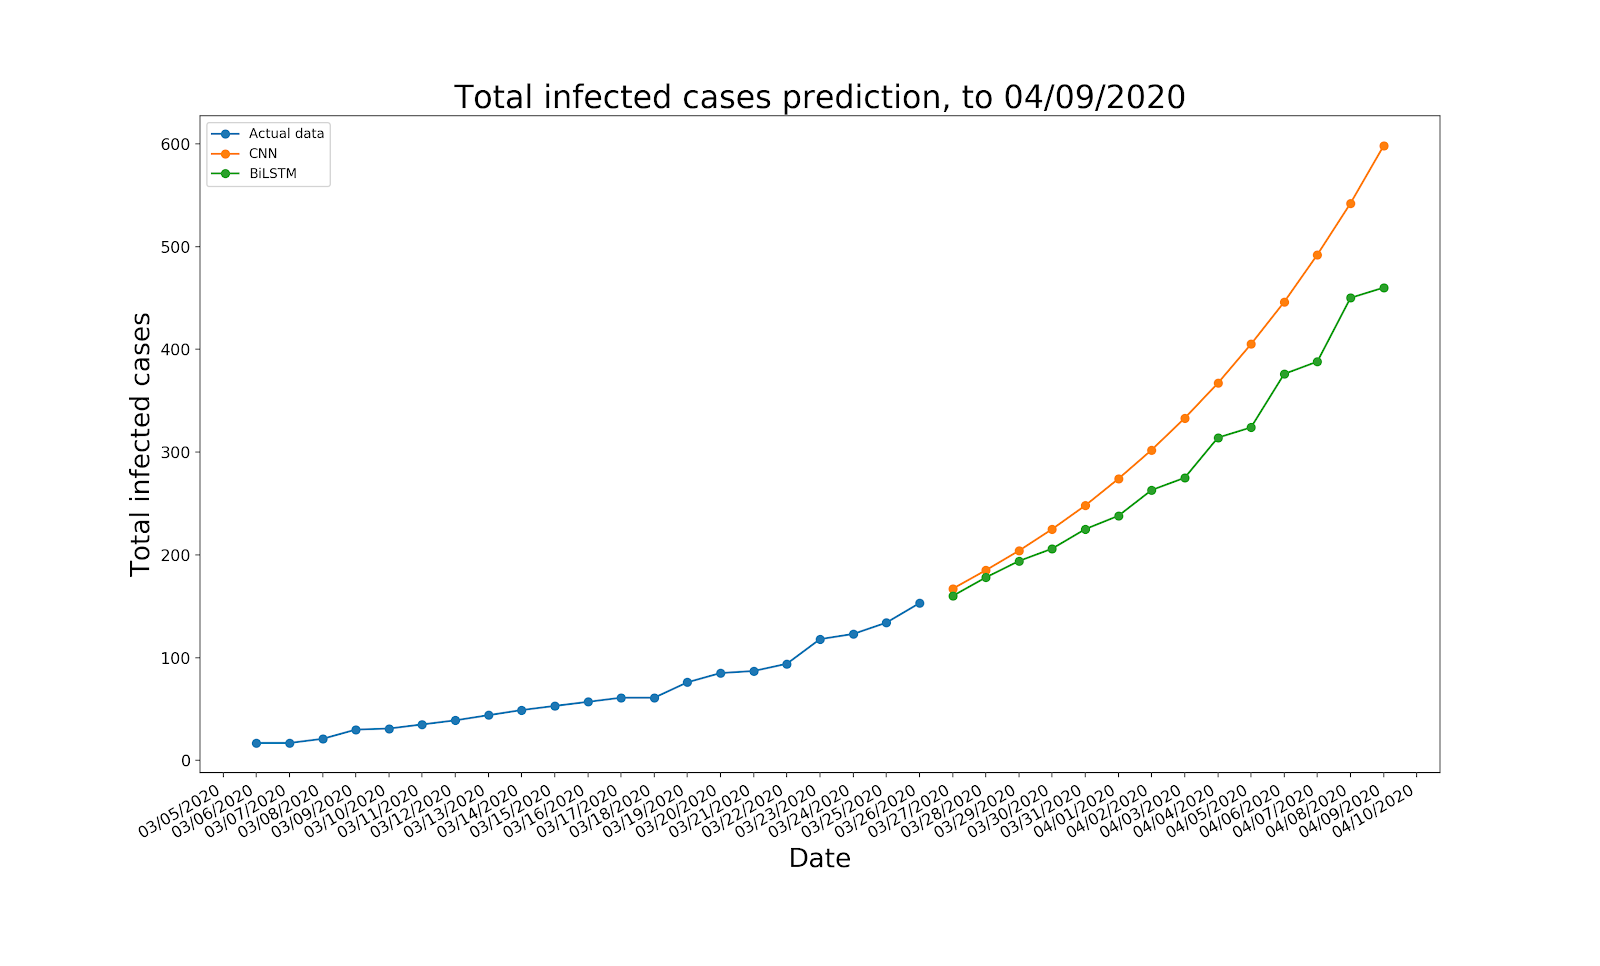
\includegraphics[scale=0.2]{cnn.png}
    \caption{Mô hình CNN và LSTM được áp dụng}
    \label{fig:cnnLSTM}
    \end{figure}
    
    \begin{figure}
    \centering
    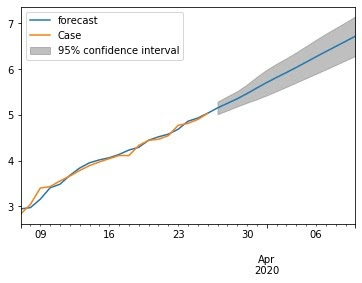
\includegraphics[scale=0.5]{arima.jpg}
    \caption{Mô hình ARIMA được áp dụng}
    \label{fig:arima}
    \end{figure}
    
    \begin{figure}
    \centering
    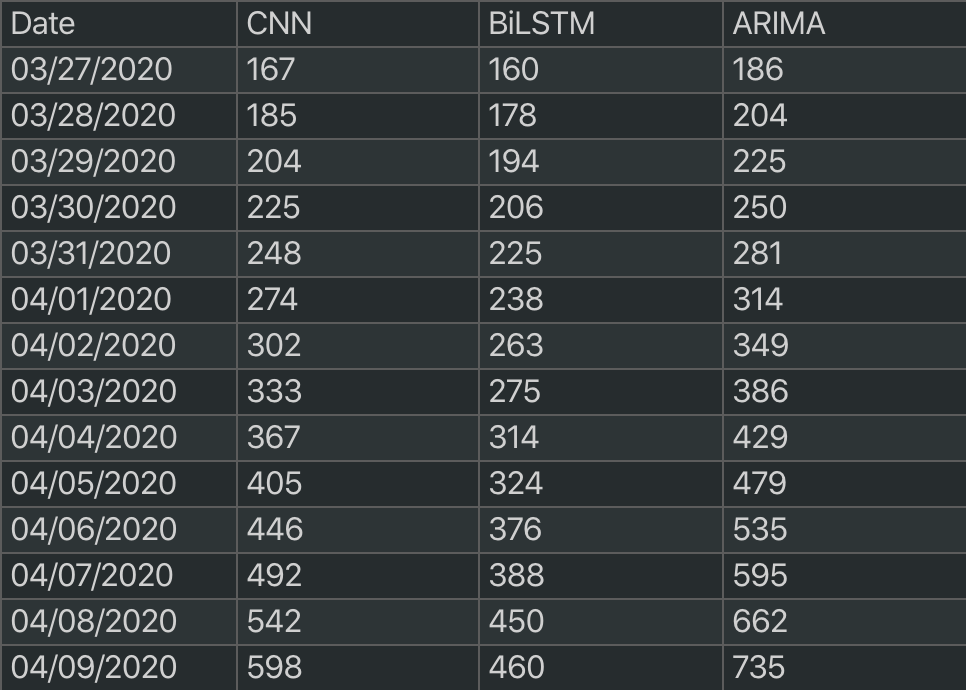
\includegraphics[scale=0.25]{data.png}
    \caption{Kết quả dự đoán của các mô hình Machine Learning truyền thống}
    \label{fig:mldata}
    \end{figure}
    
\subsection{Kết quả}

\begin{enumerate}
    \item Không xuất hiện overfit khi sai số có xu hướng nhỏ dần.
    \item Có sai số lớn vào những ngày nhất định (vào các ngày 10/03/2020 và 19/03/2020).
    \item CNN dự đoán xu hướng tăng theo cấp số nhân, LSTM dự đoán có xu hướng theo ngày.
    \item ARIMA dự đoán với sai số 5\%, và lệch $\pm 2$ ngày 
    \item Với data vào ngày 27/03/2020, dự đoán kết quả là 160-166 ca, kết quả chính xác là 163 ca, theo Bộ Y Tế \cite{govcov}.
    \item Với data vào ngày 28/03/2020, dự đoán kết quả là 176 - 180 ca, kết quả chính xác là 174 ca, theo Bộ Y Tế.
\end{enumerate}

\section{Mô hình toán học}

\subsection{Mô tả Grey Systems \& Extensions}

\begin{itemize}
    \item Ý tưởng dựa trên sự discretize theo thời gian của 1 phương trình vi phân.
    \item Đã được đề cập trong bài nghiên cứu của tác giả \cite{rongbm}
    \item Bao gồm: GM(1,1), NGBM(1,1), Optimized NGBM(1,1), Rolling optimized NGBM(1,1).
\end{itemize}

    \begin{figure}
    \centering
    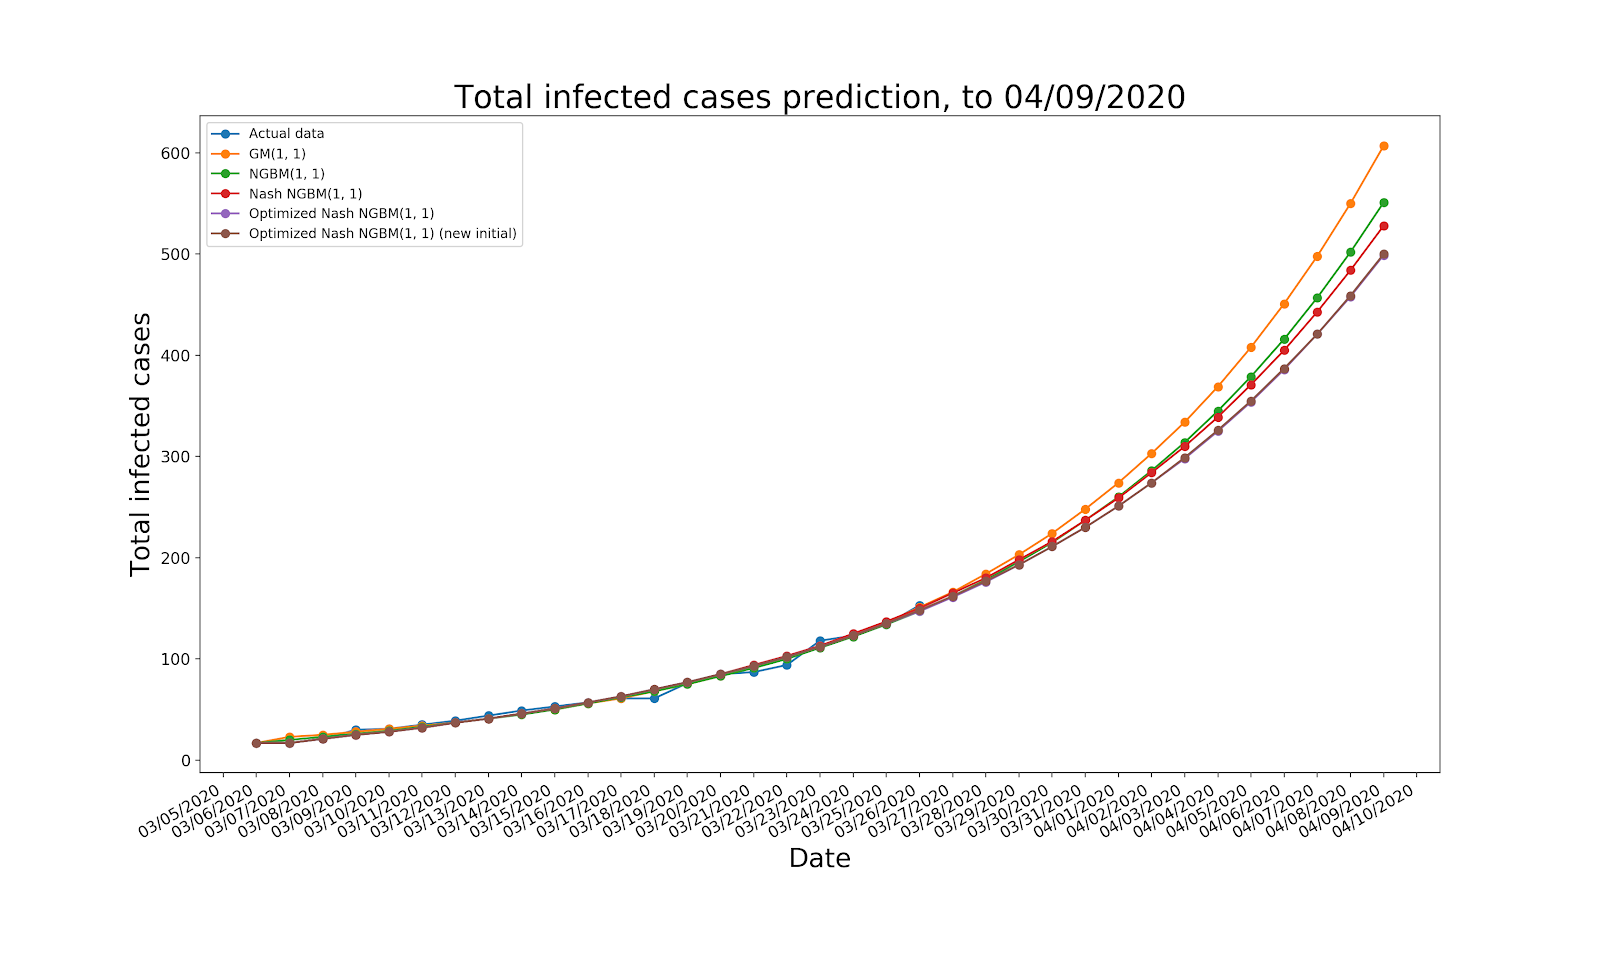
\includegraphics[scale=0.2]{grey.png}
    \caption{Áp dụng Grey Systems}
    \label{fig:gs}
    \end{figure}

    \begin{figure}
    \centering
    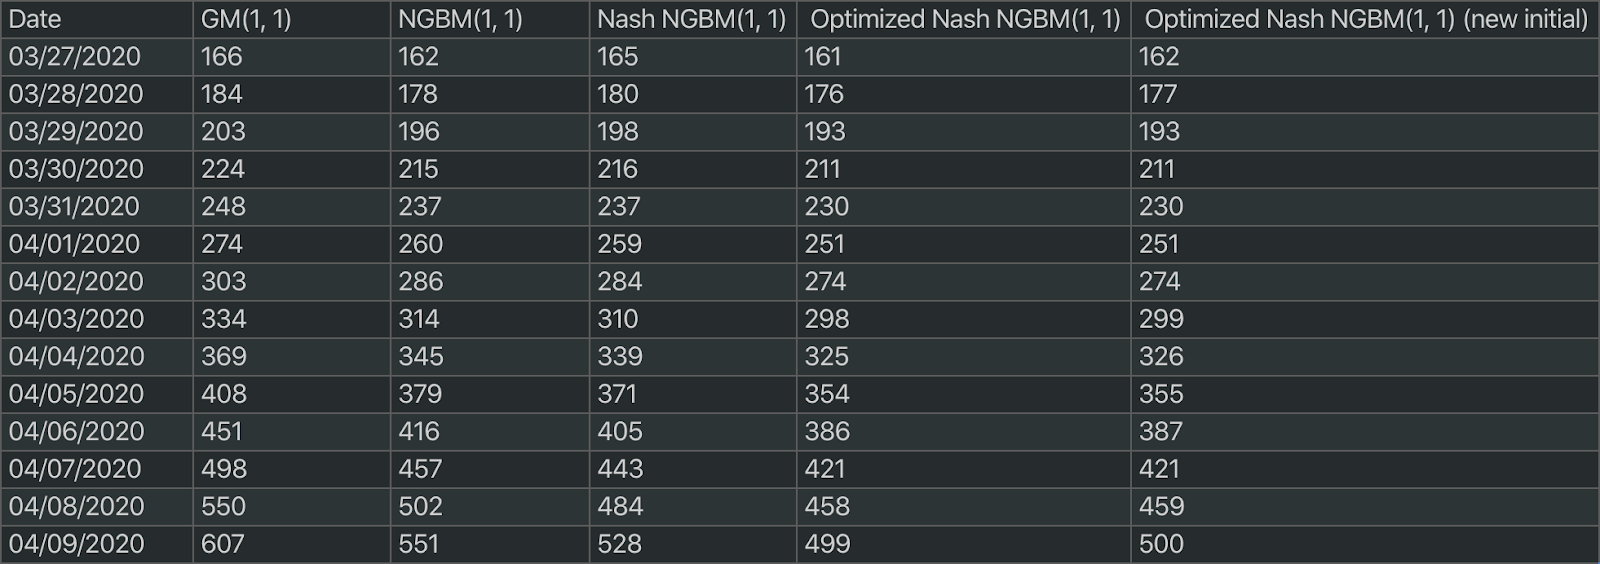
\includegraphics[scale=0.2]{greyData.png}
    \caption{Kết quả dự đoán của các mô hình Grey Systems}
    \label{fig:gsdata}
    \end{figure}

\subsection{Kết quả}

\begin{enumerate}
    \item Không xuất hiện overfit khi sai số có xu hướng nhỏ dần.
    \item Có sai số lớn vào những ngày nhất định (cụ thể ngày 4/3 và ngày 19/3).
    \item Sai số trung bình nhỏ (nhỏ hơn 5\% với những mô hình tối ưu hóa, ngày cuối cùng có sai số khoảng 3\%).  
    \item Với data mới nhất hiện có (ngày 27/3/2020), dự đoán kết quả là 160-166 ca, kết quả chính xác ngày 27/3/2020 là 163 ca, theo Bộ Y Tế \cite{govcov}.
\end{enumerate}

\section{Kết quả \& Tổng kết}

\subsection{Dự đoán chung}

Các dự đoán có thể phân loại thành 3 trường hợp theo thứ tự tình trạng xấu dần: Best Scenario (Tốt nhất), Arverage Scenario (Trung bình), Worst Scenario (Tệ nhất):

\begin{tabular}{llll}
    \textbf{Ngày} & \textbf{Best Scenario} & \textbf{Average Scenario} & \textbf{Worst Scenario} \\
    \hline
    31/03 &  225 & 230-235 & 240 \\
    09/04 (sau 2 tuần) & 450-500 & 500-550 & 600\\
\end{tabular}

\subsection{Hướng đi tiếp theo}

\begin{itemize}
    \item  Mở rộng số lượng và phạm vi mô hình áp dụng.
    \item Sử dụng mô hình đa biến để các mô hình mang thêm ý nghĩa dịch tễ.
    \item Ngoài dự đoán số ca mắc của địa phương/cả nước, có thể dùng Machine Learning để dự đoán ca bệnh (xác suất phải dùng ICU, tử vong/hồi phục, ngày xuất viện,...)
\end{itemize}

\pagebreak

\begin{thebibliography}{}

\bibitem{govcov} 
https://ncov.moh.gov.vn/. 
\textit{Thống kê tình hình dịch bệnh COVID-19}. 
Bộ Y Tế, Việt Nam, 2020.

\bibitem{rongbm}
HA, Ngo, TN, Hoang.
\textit{A rolling optimized nonlinear grey bernoulli model ROMGBM(1,1) and application in predicting total 2019-nCoV infected cases}.
2020.
\end{thebibliography}

\end{document}
